\section{Results}

\subsection{BERT Fine-Tuning Partial \& Full Epochs}

In order to establish a baseline performance, we fine-tuned BERT for up to 6 epochs with results shown in Figure [\ref{fig:QnABertPerformance}]. We measure performance for every 10th of a fractional epoch between 0 and 1 epochs, as well as full epochs up to 6. We observed that performanced peaked at 2 epochs, achieving an Exact Match (EM) of 0.747, and an F1 score of 0.792. Between 0 and 1 epochs, performance consistently increased both in terms of EM and F1. For comparison with other published works, see Appendix. \\

In order to select where to extract our hidden state activations, we chose 2 time points to balance training time and model performance. The first is a full training epoch. On our GPU, fine-tuning for 1 epoch is expensive and takes around 5 hours, but performance is already relatively decent compared to peak performance at 2 epochs. This time point gives us high quality embeddings for model development. The second time point is 3/10 of an epoch, which takes about 1.5hr to fine-tune. While cheaper, at this time point, the model has yet to achieve the large jump in performance observed between 3/10 and 4/10 of an epoch. This provides us an opportunity for improvement using our models. 

\begin{figure}[ht]
	\centering
	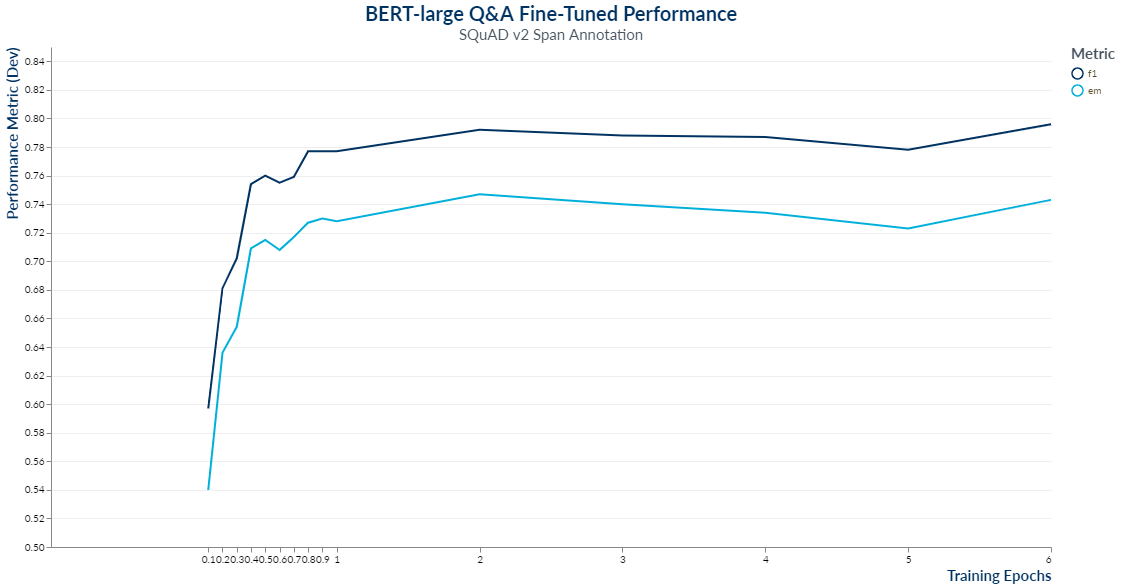
\includegraphics[width=75mm]{images/QnA_BERT_Training_Performance_plot.png}
	\caption{\label{fig:QnABertPerformance}QnA Performance, BERT SQuAD 2.0}
\end{figure}

\subsection{Models trained at 3/10 epoch BERT embeddings}

Using the embeddings at 3/10 of epoch, we explored over 20 parameter-efficient models using a combination of CNNs, pooling and compression techniques. Table [?] shows the performance of our most promising models, and results of all models are in the Appendix. \\

First, we compared two pooling strategies. Our LP (learned pooling) model is identical to the pooling model outlined in Tenney et. al. [?], where weights for combining each encoder layer is learned. The AP (average pooling) model proposed by Ma et. al. [?] on the other hand weights each encoder layer equally. We found that an LP model achieved similar performance as BERT itself, while average pooling significantly decreased performance. An analysis of the learned weights suggests that a non-uniform distribution of pooling weights is optimal, with the distribution slightly favoring later layers of BERT compared to earlier layers (see Appendix). \\

Next, we evaluated the possibility of using adapters modified from Houlsby et. al (see Methods). We found that our modified adapters of all flavors improved model performance compared to baseline BERT. Our best model uses an adapter of size of 386 with weight sharing enabled for each encoder layer, achieving an EM of 0.699 and F1 of 0.740. A skip connection between the final encoder layer and our model’s penultimate hidden layer is also included (see Figure [?]). Without weight-sharing, the number of parameters increases by about 24x, and model performance slightly decreases. While Houlsby et. al. found that an adapter size of 64 provides the best F1 score when used in between transformer blocks, for our purposes, a size of 64 performed worse with or without weight-sharing. Our best adapter model significantly beats BERT fine-tuned to the same level of 3/10 of an epoch by about 4 percentage points in both EM and F1, although we failed to reach performance at 1 full epoch. \\

While we extensively explored stacking pooling with adapters and CNNs, we did not find a model which performed better than our best adapter model. For example, Table [\ref{tbl:3_10_Models}] shows a model where we stacked learned pooling with our best adapter model and abbreviated Xception network. The number of parameters increased by 16x, but performance was no better than pooling alone.

\begin{table}[ht]
	\centering
	\small
	\begin{tabular}{L{3.5cm} C{0.6cm} C{0.6cm} C{0.6cm} C{0.6cm}}
		\hline
		\textbf{Model} (\% params of $BERT_{LARGE}$)       & \textbf{EM $\frac{3}{10}e$} & \textbf{F1 $\frac{3}{10}e$} & \textbf{EM $1e$} & \textbf{F1 $1e$}\Tstrut \\
		\hline
		BERT $\frac{3}{10}e\;\left(100\%\right)$           & $0.654$ & $0.702$ & $0.728$ & $0.777$\Tstrut\Bstrut  \\
		BERT $1e\;\left(100\%\right)$ 					   & $0.670$ & $0.712$ & $0.728$ & $0.777$\Tstrut\Bstrut  \\
		learned pooling $\left(0.001\%\right)$             & $0.660$ & $0.703$ & $0.725$ & $0.759$\Tstrut\Bstrut  \\
		average pooling $\left(0.001\%\right)$             & $0.657$ & $0.700$ & $0.736$ & $0.741$\Tstrut\Bstrut  \\
		\hline\hline
		adapter shared 386 skip $\left(0.124\%\right)$     & \boldmath$0.699$ & \boldmath$0.740$ & \boldmath$0.745$ & \boldmath$0.791$\Tstrut\Bstrut  \\
		\hline\hline
		adapter independent 386 $\left(2.957\%\right)$     & $0.676$ & $0.723$ & $0.730$ & $0.778$\Tstrut\Bstrut  \\
		adapter shared 64 $\left(0.021\%\right)$           & $0.680$ & $0.732$ & $0.722$ & $0.761$\Tstrut\Bstrut  \\
		adapter independent 64$\left(0.491\%\right)$         & $0.684$ & $0.716$ & $0.736$ & $0.782$\Tstrut\Bstrut  \\
		pooling adapter 386 \& xception $\left(1.970\%\right)$         & $0.668$ & $0.711$ & $0.699$ & $0.751$\Tstrut\Bstrut  \\
		\hline
	\end{tabular}
	\caption{\label{tbl:3_10_Models}Models at $\frac{3}{10}$ epochs but evaluated at 1 epoch}
\end{table}

\subsection{Best Models on top at 1 epoch}

Using the embeddings at 1 epoch of fine-tuning, we trained the same set of 20 models as at 3/10 of an epoch of fine-tuning (see the Appendix for a full set of results). In most cases, we found that our models outperformed BERT at 1 epoch of fine-tuning. One exception is our adapter 386 model with independent weights, which suffered about 1 percentage point drop. Table [\ref{dev_set_performance}] shows that adapter models of size 64, with or without weight-sharing, both beat BERT, but the best model found is almost identical to that found at 3/10 of an epoch utilizing an adapter size of 386. The only exception that a skip connection is not needed in this case. This model’s performance is also competitive with maximum performance achieved with BERT fine-tuning, with a slightly improved EM (0.749 vs 0.747) and a slightly decreased F1 (0.790 vs 0.792). This result shows that we are able to reduce BERT fine-tuning by 1 epoch and still achieve similar performance with a model of only about 0.124\% of the number of BERT parameters. 

\begin{table}[ht]
	\centering
	\small
	\begin{tabular}{L{2.8cm} L{1.8cm} C{0.6cm} C{0.6cm}}
		\hline
		\textbf{Model} & \textbf{\% params of} $BERT_{LARGE}$ & \textbf{EM} & \textbf{F1}\Tstrut \\
		\hline
		BERT $1e$ & 100\% 						 & $0.728$ & $0.777$ \\
		BERT $2e$ (\textit{best}) & 100\%		 & $0.747$ & $0.792$ \\
		adapter shared 386 & 0.124\% 			 & $0.749$ & $0.790$ \\
		\hline\hline
		adapter independent 386 & 2.957\% 		 & \boldmath$0.716$ & \boldmath$0.767$ \\
		\hline\hline
		adapter shared 64 & 0.021\% 			 & $0.739$ & $0.785$ \\
		adapter independent 64 & 0.491\% 		 & $0.736$ & $0.784$ \\
		tenney adapter 386 \& xception & 1.970\% & $0.741$ & $0.786$ \\
		\hline
	\end{tabular}
	\caption{\label{tbl:dev_set_performance}Dev set performance}
\end{table}

\subsection{Performance of models trained at 3/10 epoch on higher quality embeddings}

We wanted to better understand why models trained on embeddings derived at 1 epoch of fine-tuning performed better than models trained on embeddings derived at 3/10 of an epoch. In order to do this, we took all of our models trained on the 3/10 embeddings, and evaluated their performance on the dev set with embeddings derived at 1 epoch. To our surprise, all models experienced a significant jump in performance compared to evaluation at embeddings derived at 3/10 of an epoch. Figure [?] shows a comparison of these results on our top models, and Appendix S[?] contains data for all models.  \\

For example, our best model trained at 3/10 of an epoch achieved a performance of 0.745 EM and 0.791 F1 when evaluated on embeddings from 1 epoch. This is a significant boost compared to evaluating the exact same model on embeddings derived from 3/10 of an epoch (0.699 EM and 0.740EM). This model performs similarly to our best model trained on 1 epoch embeddings, and by a transitive relation, also performs similarly to maximum BERT performance at 2 epochs. We consider this a significant achievement for a model that has only seen data from 3/10 of an epoch of fine-tuning. \\

Our result suggests that models trained at 3/10 of an epoch are learning transformations that are transferable even as BERT is further fine-tuned. This implies that BERT is maintaining some level of constancy in the structure of its internal representations. Practically, this means that our models can be trained in parallel with BERT fine-tuning. As BERT learns better internal representations of the data, models trained on earlier representations can leverage this improvement and achieve better performance on the task on hand. \\

\subsection{Training with less data}

The previous sections show that our models perform well compared to BERT when trained on the full dataset. However, since supervised data can be difficult to obtain for certain tasks, we wanted to explore whether our models can perform well with significantly less data. In addition in our case, since embeddings can be expensive to calculate and store, reducing training data also helps with our data management issue (see Methods). To answer this question, we trained our best models (for both 3/10 epoch and 1 epoch embeddings) on varying amounts of data, ranging from 0\% to 100\% of the dataset at step sizes of 10\%. All models were trained for 1 epoch, the same as using the full dataset. Here, 0\% represents randomized weights with no training. For the model at 3/10 of an epoch, we measured its dev set performance on both the 3/10 epoch embeddings and 1 epoch embeddings.  \\

Figure [\ref{fig:1_epoch_embeddings__adapter_386_with_skip}] shows the results. In all cases, we rapidly approach strong performance early on, beating BERT at around 30\% of the data. Even at 10\% of the data, we are only about 3 percentage points in terms of EM, and 2 from F1, from maximum peak performance. This shows that we can in fact achieve strong performance even when using training less. 

\begin{figure}[ht]
	\centering
	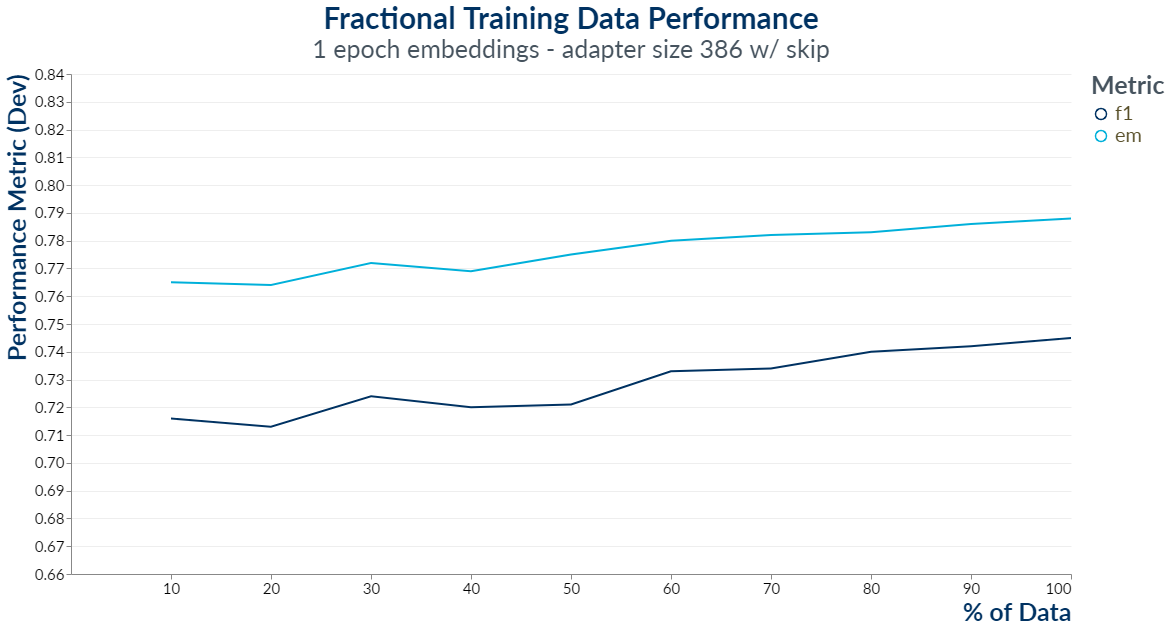
\includegraphics[width=75mm]{images/1_Epoch_Embeddings__Adapter_386_with_Skip.png}
	\caption{\label{fig:1_epoch_embeddings__adapter_386_with_skip}1 epoch embeddings - adapter 386 w/ skip}
\end{figure}

\begin{table}[ht]
	\centering
	\small
	\begin{tabular}{L{0.8cm} C{0.90cm} C{0.90cm} C{1.5cm} C{1.5cm}}
		\hline\Bstrut
		\textbf{\% data} & \textbf{EM} & \textbf{F1} & \textbf{EM \boldmath$1e$ embeddings} & \textbf{F1 \boldmath$1e$ embeddings}  \\
		\hline\Tstrut\Bstrut
		10\%  & $0.633$ & $0.692$ & $0.712$ & $0.768$ \\[.1cm]
		20\%  & $0.633$ & $0.690$ & $0.714$ & $0.767$ \\[.1cm]
		30\%  & $0.660$ & $0.711$ & $0.735$ & $0.782$ \\[.1cm]
		40\%  & $0.663$ & $0.695$ & $0.737$ & $0.775$ \\[.1cm]
		50\%  & $0.673$ & $0.712$ & $0.741$ & $0.783$ \\[.1cm]
		60\%  & $0.681$ & $0.719$ & $0.733$ & $0.772$ \\[.1cm]
		70\%  & $0.683$ & $0.729$ & $0.731$ & $0.779$ \\[.1cm]
		80\%  & $0.686$ & $0.724$ & $0.741$ & \boldmath$0.785$ \\[.1cm]
		90\%  & $0.687$ & $0.734$ & $0.733$ & $0.783$ \\[.1cm]
		100\% & \boldmath$0.689$ & \boldmath$0.733$ & \boldmath$0.736$ & $0.783$ \\[.1cm]
		\hline
	\end{tabular}
	\caption{\label{tbl:3_10_embeddings__adpater_386}$\frac{3}{10}$ Epochs embeddings - adapter 386}
\end{table}


